% !Mode:: "TeX:UTF-8"
\chapter{云辅助的车辆网络功率控制与任务卸载} \label{chap:table}  %\cite{yaojianquan2009}

\section{引言}\label{section3-1} \label{chap:introduction}
云辅助移动边缘计算(C-MEC)为车载网络提供了丰富的计算资源,是一种前景广阔的任务卸载解决方案。本文提出了一种稳健的功率
控制和任务卸载方案,以卸载计算任务并最大化 C-MEC 网络的效用。然而,不确定的信道状态会严重影响卸载任务的传输稳定性。为了模拟信道的不确定性,采用了一阶马尔可夫过程,并考虑了车辆的移动性。此外,由于频谱资源有限,假设信道重用会导致复杂的同信道干扰。为了克服这些限制,对信号链路实施了概率约束,以确保通信质量。采用伯恩斯坦近似法将原始约束转化为可解约束。此外,还进一步采用了块坐标下降(BCD)方法和连续凸近似(SCA)技术来解决非凸鲁棒性优化问题。为确定最优解,提出了一种鲁棒电源控制和任务卸载调度算法。对提出的算法进行了数值模拟,以评估系统的性能。结果表明,与基准模型相比,该算法非常有效,尤其是在信道不确定的通信环境中。
移动边缘计算(MEC)和移动云计算(MCC)是新兴5G网络的两种新架构。
移动边缘计算(MEC)和移动云计算(MCC)作为新兴的5G网络的两种新架构,通常用于支持物联网设备的任务卸载、
特别是提供低延迟、高可靠性的计算服务。在网络中心的边缘,MEC可以减少传输延迟,并为车辆分配计算资源,以缓解计算压力
\cite{CCO}。
然而,当计算任务要求较高时,MEC的计算资源仍显不足。由于高性能计算由云服务器提供,基于云的计算网络已被部署以满足爆炸式增长的计算卸载需求。然而,云计算中心往往远离主干道,导致云计算延迟较长。
\cite{Qian2023}.
在高动态车联网中,车辆传输的数据必须实时处理。因此,在网络架构中部署C-MEC,以提供丰富的计算资源并减少传输延迟。
\section{系统模型与问题描述}\label{section3-2}
本文研究的C-MEC车载网络如图 \ref{F1}所示,由MEC层和云计算层分层计算卸载架构组成。众多车辆在RSU的覆盖范围内被划分为多个地理区域,每个RSU下覆盖一个小区,每个RSU配备一台MEC服务器,为车辆提供计算卸载服务。我们将移动系统中的两组车辆和MEC服务器分别记为$\mathcal{V}=\left\{1,2,..., V\right\}$和$\mathcal{M}=\left\{1,2,..., M\right\}$。高速移动无线通信链路称为 V2RSU(V2R)链路,固定有线连接链路称为 RSU 到云(R2C)链路。详细的卸载过程描述如下。首先,车辆通过无线接口向云发送卸载请求信息,其中包括所需的通信资源、任务 ID 和提交时间,以及任务的最大可容忍服务时间。其次,MEC 服务器根据接收到的请求信息进行调度,包括任务上传服务器和任务计算服务器。最后,任务上传后,任务被推送到服务器队列中,直到服务器执行任务。
%此外,本文中使用的一些术语如表所示。
\begin{figure}[H]
\centering
\includegraphics[width=14cm]{figures//chap3//model2.eps}
\caption{System m}
\label{F1}
\end{figure}

\subsection{通信模型}\label{section3-2-1}
由于车辆移动速度快,通信模式与传统的蜂窝通信不同。因此,很难直接获得 CSI。其中,RSU 仅能准确获取车辆到 RSU 链路的大尺度衰落 $L^2$,而小尺度衰落 $h$ 受多普勒效应引起的快速信道变化影响较大。我们假设CSI是通过信道估计获得的,因此,我们利用一阶高斯-马尔可夫过程\cite{Kim2011}对每个传输时间间隔内的小尺度衰落信道估计$h$建模如下,
\begin{eqnarray}\label{E1}
h=\xi{\widetilde{h}}+\sqrt{1-\xi^2}\zeta.
\end{eqnarray}
我们假设估计的信道增益 $\widetilde{h}$ 表示对 $h$ 的估计,${\widetilde{h}}^2$ 是指数分布,具有单位平均值\cite{Sakr2014}。此外,$\xi\in\left(0,1\right)$ 表示 V2R 链路上的相关系数,$\zeta$ 表示信道增益,其复高斯分布为 $\zeta\sim CN\left(0,\delta^2\right)$ ,与 $\widetilde{h}$ 无关。系数$\left(0<\zeta<1\right)$量化了两个连续时隙之间的信道相关性,我们假设所有车辆都存在相同的时间相关系数$\zeta$。Jakes的衰落信道统计模型\cite{Kim2011}指出:$\zeta=J_0\left(2\pi f_{max}T_s\right)$ ,其中$J_0$是第一类零阶贝塞尔函数。$f_{max}=\bar{\nu}f_c/c $ 是最大多普勒频率,其中 $\bar{\nu}$ 表示车辆速度,$f_c$ 表示 5.9 Ghz 的载波频率,$c=3\times{10}^8$m/s,$T_s$ 是周期反馈延迟。发射车和 RSU 都知道实际的 $\zeta$。

根据上述讨论,从第$ i$ 个车辆发射器到第 $j $个接收器的第$ k $个时隙内,有效链路和干扰链路的移动 V2R 信道功率增益用共享表达式表示:
\begin{eqnarray}\label{E2}
G_{i,j}^k={\widetilde{g}}_{i,j}^k+{\hat{g}}_{i,j}^k,
\end{eqnarray}
其中 ${\widetilde{g}}_{i,j}^k=L_{i,j}^2{\widetilde{h}}_{i,j}^2\xi_{i,j}^2$ , ${\hat{g}}_{i,j}^k=L_{i,j}^2\left(1-\xi_{i,j}^2\right)\zeta_{i,j}^2\ $ ,$ {L_{i、 j}^k}^2 $
表示第 $k $ 个时隙的大规模衰减效应,包括阴影衰减和从道路上第 $i$ 个车辆发射器到第 $ j $ 个接收器的路径损耗。此外,${\hat{g}}_{i,j}^k$ 是观测值,${\widetilde{g}}_{i,j}^k$ 表示指数随机变量,参数为 $\frac{1}{L_{i,j}^k}^2({1-{\zeta_{i,j}^k}^2}) $ ,该参数基于 \cite{Xie2020}。

为了提高频谱利用率并实现多车联合通信,V2R 通信重复使用同一上行链路信道。换句话说,车辆 $j$ 和车辆 $i$ 共享同一个上行链路信道,从而导致它们之间产生干扰。在这种情况下,V2R 链路的信号干扰加噪声比(SINR)计算公式为,
\begin{eqnarray}\label{E3}
\gamma_i\left(\mathbf{p}\right)=\frac{p_ig_{i,j}}{{\sum_{j=1,j\neq i}^{M}{p_jg_{j,i}}+\sigma^2}},
\end{eqnarray}
其中,$p_j$ 表示第 j 个发射器车辆的发射功率,$\sigma^2$ 为背景噪声。因此,根据香农定理计算出车辆的确定性等效传输速率为,
\begin{eqnarray}\label{E4}
{R_i\left(\mathbf{p}\right)=\log}_2{\left(1+\frac{p_ig_{i,j}}{\sum_{j=1,j\neq i}^{M}{p_jg_{j,i}}+\sigma^2}\right)}.
\end{eqnarray}
当输入参数为 $d_{i,up}$ 时,车辆 $i$ 向上行链路发送任务输入时的传输时间定义为 $t_{i,up}$。

因此,每个 V2R 链路的上传时间可表述为,
\begin{eqnarray}\label{E6}
t_{i,up}=\frac{d_{i,up}}{WR_i\left(\mathbf{p}\right)},,
\end{eqnarray}
其中,$W$ 表示多个 V2R 链路重复使用的信道带宽,$d_{i,up}$ 表示输入数据的大小,包括系统设置、程序代码和输入参数,这些数据是程序执行时必须传输的。

通信传输延迟是影响车载网络性能的一个重要因素 \cite{RAI}。 到 RSU 的数据包在传输前必须进入队列,其中传输速度为 $R_i$。第i个V2R接收器的数据包到达过程遵循参数为$k_i$的泊松过程,数据包长度为参数为$\tau_i$的指数分布。由于基于$M/M/1$队列的方法可以保证车辆通信的可靠性,我们利用$M/M/1$模型对系统进行分析,并将预期时延表示为第i条V2R链路传输速率的函数,其表达式如下,
\begin{eqnarray}\label{E7}
D_i=\frac{1}{{\tau_iR}_i-k_i}.
\end{eqnarray}

\subsection{车辆计算模型}\label{section3-2-2}
我们将处理车辆 $i$ 的 1 位输入数据所需的 CPU 周期数表示为 $c_0$ \cite{Zhang2017},它不可分割,无法分解为更小的组件 \cite{Saleem2021}。
我们认为,在$ \mathcal{V}$ 中,每辆车每次都有不同的计算任务,记作 $T_i$,由两个参数组成的元组来定义,即 $\langle d_{i,up}, c_{i,e}\rangle$,其中 $c_{i,e}$ [cycles] 指定了工作量 \cite{Tran2019}。因此,完成任务的计算成本 $c_{i,e}$ 可以通过 $c_{0}*d_{i,up}$ 得到。每个任务都被卸载到 MEC 服务器,然后传输到云服务器。通过将计算任务卸载到 MEC 服务器,车辆可以获得更多计算资源。然而,在上行链路方向传输任务输入可能会消耗额外的时间。

每个 RSU 上的 MEC 服务器按时段为车辆提供计算卸载服务。计算资源由固定速率 $\bar{f}$(即每秒 CPU 周期数)量化。第 i 辆车将每个任务的输入数据上传到最近的 RSU。RSU 首先处理小规模、对延迟敏感的数据,然后将剩余数据转发给远程云服务器。{云服务器同时为多个 RSU 提供计算服务。RSU 可用的计算资源取决于从云服务器分配的计算速率 $f_i$,}即每秒 CPU 周期数。因此,计算卸载造成的延迟可计算为,
\begin{eqnarray}\label{E8}
t_{i,exe}=\frac{c_{i,e}}{\bar{f}+f_i}.
\end{eqnarray}
\subsection{问题的定义}\label{section3-2-3}
\begin{comment}
\begin{table}[htbp!]
 \centering\small
 \Tablecaption{燕山大学硕士学位论文参考文献规则}\label{tab:ysubof}
\begin{tabular}{llr}
 \toprule
    论文版本    & 参考文献标准    & 实施年份(年)  \\
 \midrule
    旧版        & BF7714-87       & 1987            \\
    新版        & GBT7714-2005    & 2005            \\
 \bottomrule
 \end{tabular}
\end{table}
\end{comment}
如果计算速度为 $f_i$,则车辆 $i$ 因卸载而产生的总延迟时间为,
\begin{eqnarray}\label{E9}
 t_i=\frac{c_{i,e}}{\bar{f}+f_i}+T_c,
\end{eqnarray}
其中,云服务器和 RSU 之间的传输延迟定义为 $T_c$,通常设为一个常量 \cite{Xiao2020}。因此,任务完成时间的相对效用函数的特征为,
\begin{eqnarray}\label{E10}
U_{i,exe}=\frac{t_{max}-t_{i,exe}}{t_{max}},
\end{eqnarray}
其中,$t_{max}$ 为{任务完成可容忍阈值的最长时间}。换句话说,当任务同时在 MEC 服务器和云上执行时,每辆车都能通过最小化任务执行时间获得更大的效用。否则,就会产生相应的损失。因此,车辆 $i$ 的卸载效用定义为 $\frac{U_{i,exe}}{t_{i,up}}$,即单位时间内的卸载效用函数。

本节将功率控制和任务卸载表述为一个优化问题,试图最小化网络中所有车辆由延迟和传输速率组成的总系统成本。给定上行链路功率分配向量 $\mathbf{p}$ 和计算速率向量 $\mathbf{f}$ 后,系统效用被定义为所有车辆卸载效用的加权和。
\begin{eqnarray}\label{E12}
U=\sum_{i=1}^{M}\frac{U_{i,exe}}{t_{i,up}},
\end{eqnarray}
其中,$U$ 是更大的执行时间效用,上传时间成本较小。我们将稳健优化问题,即电源控制和任务卸载问题,表述为系统效用最大化问题,
\begin{align}
& \max\limits_{\mathbf{p},\mathbf{f}}\sum_{i=1}^{M}\frac{U_{i,exe}}{t_{i,up}}                                   \label{E3-13}\\
\text { s.t. }
& \textrm{Pr}\left\{\gamma_i\geq\gamma_{th}\right\}\geq1-\varepsilon_1,                                         \tag{\ref{E3-13}{-1}}      \label{E3-13-1}\\  %信噪比中断概率约束
& \textrm{Pr}\left\{\frac{1}{\tau_iR_i-k_i}+\frac{c_{i,e}}{\bar{f}+f_i}\le D_{max}\right\}\geq1-\varepsilon_2,  \tag{\ref{E3-13}{-2}}      \label{E3-13-2}\\  % 功率阈值
& \sum_{i=1}^{N}f_i\le f_{total},                                                                               \tag{\ref{E3-13}{-3}}      \label{E3-13-3}\\  %时隙分配加起来是一
& 0\le p_i\le p_{max},                                                                                          \tag{\ref{E3-13}{-4}}      \label{E3-13-4} %这个是时隙的约束
%& q_U^{n\mathrm{\ }+1}-q_U^{n\mathrm{\ }}\le tV_{max}, \forall m         \tag{\ref{E2-13end}{-5}}      \label{E2-13end5}    %无人机飞行轨迹
\end{align}
其中,$U$ 表示网络效用。\eqref{E3-13}中的约束条件解释如下: 约束条件 \eqref{E3-13-1} 保证了车辆的 QoS 要求。然而,网络拓扑结构的时变会导致大量计算。在车辆通信场景中,实时 SINR 难以量化获取。由于 CSI 反馈的时间间隔非常小,因此用长期 SINR 代替实时 SINR。我们用 $\gamma_i$ 表示第 i 个 V2R {链路的平均 SINR,使用较小的 CSI 反馈时间间隔}。为确保任务成功卸载到 RSU,SINR 必须大于 SINR 阈值 \cite{liu2021}。$\gamma_{th}$ 是检测 V2R 链路通信的 SINR 阈值。$\textrm{Pr}\left\{\cdot\right\}$ 定义了输入 SINR 的概率。中断概率约束保证了车辆链路的可靠性。$D_{max}$ 表示第 $i$ 个 V2R 链路在数据传输过程中允许的最大延迟。此外,$\varepsilon_1$和$\varepsilon_2$分别是与SINR和延迟约束相关的中断概率阈值,其中$\varepsilon_1,\varepsilon_2\in\left(0,1\right)$。约束 \eqref{E3-13-2}表示通信和计算的总延迟大于延迟阈值。约束 \eqref{E3-13-3} 确保云服务器必须为与其相关联的 RSU 分配计算资源,约束 \eqref{E3-13-3} 还确保分配给所有相关联 RSU 的总计算资源不得超过云服务器的计算能力。因此,特定边缘云所服务的应用数量必须低于其容量。在约束条件\eqref{E3-13-4}中,$p_{max}$是车辆通信网络中发射车辆的最大发射功率,且发射功率大于零。

\begin{comment}
实现代码如下:
\end{comment}
\section{问题的求解}\label{section3-3}
在本节中,我们提出了一种基于 BCD 的算法来求解优化问题 \eqref{E3-13}。BCD 方法将复杂的原问题分解为一系列较简单的子问题。BCD 方法首先将所有变量分成两块,交替优化。

为了解决 \eqref{E3-13}问题,可以通过固定计算率向量 $\mathbf{f}$ 的优化变量来优化问题。该问题通过交替优化两个子问题来解决。去掉向量 $\mathbf{f}$ 后,问题 \eqref{E3-13-1} 可以转化为下面的问题,
\begin{align}
& \textbf{P1}:\max\limits_{\mathbf{p}}\sum_{i=1}^{M}\frac{U_{i,exe}}{t_{i,up}}                                  \label{E3-14}\\
\text { s.t. }
& \textrm{Pr}\left\{\gamma_i\geq\gamma_{th}\right\}\geq1-\varepsilon_1,                                         \tag{\ref{E3-14}{-1}}      \label{E3-14-1}\\  %信噪比中断概率约束
& \textrm{Pr}\left\{\frac{1}{\tau_iR_i-k_i}+\frac{c_{i,e}}{\bar{f}+f_i}\le D_{max}\right\}\geq1-\varepsilon_2,  \tag{\ref{E3-14}{-2}}      \label{E3-14-2}\\  % 功率阈值
& 0\le p_i\le p_{max},                                                                                          \tag{\ref{E3-14}{-3}}      \label{E3-14-3}  %\\  %时隙分配加起来是一
%& 0\le p_i\le p_{max},                                                                                          \tag{\ref{E3-13}{-4}}      \label{E3-13-4} %这个是时隙的约束
%& q_U^{n\mathrm{\ }+1}-q_U^{n\mathrm{\ }}\le tV_{max}, \forall m         \tag{\ref{E2-13end}{-5}}      \label{E2-13end5}    %无人机飞行轨迹
\end{align}

\subsection{目标方程中的连续凸逼近方法}\label{section3-3-1}
由于$t_{i,up}$中的香农定理的形式,目标函数\eqref{E3-14}是对数形式,因此\eqref{E3-14-1}是一个非凸和非确定多项式困难(NP-hard)问题。这里使用 SCA 方法将问题 \eqref{E3-14-1} 简化为可解问题。利用近似约束来近似原始函数如下,
\begin{eqnarray}\label{E15}
\begin{array}{ll}
\alpha \ln{\left(z\right)}+\beta\le \ln{\left(1+z\right)},\\
\end{array}
\end{eqnarray}
其中 $\alpha=\frac{z_0}{1+z_0}$ 并且 $\beta=\ln{\left(1+z_0\right)}-\frac{z_0}{1+z_0}\ln{\left(z_0\right)}$。 \eqref{E15}中的每个项都可以通过连续凸近似转换为 $A_k\ln\left(\gamma_k\left(e^{\widetilde{\mathbf{p}}}\right)\right)+B_k$ 。 其中,$A_k$和$B_k$分别选为$A_k=\gamma_i/\left(1+\gamma_i\right)$和$B_k=\ln{\left(1+\gamma_i\right)}-A_k\ln{\left(\gamma_i\right)}$,其中$A_k=1$,$B_k=0$。目标函数的每项都可以写成如下,
\begin{eqnarray}\label{E16}
\frac{1}{\ln{2}}\sum_{i=1}^{M}{\frac{U_{i,exe}}{d_{i,up}}\left.\left[{A_k\ln{\left(\gamma\left(p\right)\right)}+B}_k\right.\right]},
\end{eqnarray}
由于 \eqref{E3-14} 中的目标函数是 SINR 的分数,因此不容易直接计算。因此,我们使用变量替换法,即 ${\hat{p}}_i=\ln{p_i}$,
$p_i=e^{{\hat{p}}_i}$, and ${\hat{p}}_i\le \ln{p_{max}},\ \forall\ \ 1\le i\le M$
\begin{eqnarray}\label{E17}
U=\max\frac{1}{\ln{2}}\sum_{i=1}^{M}\left.\frac{U_{i,exe}}{d_{i,up}}\left[{A_k\ln{\left(\gamma\left(e^{\widetilde{P}}\right)\right)}+B}_k\right.\right].
\end{eqnarray}

\begin{comment}
\begin{table}[htbp!]
\centering\small
\Tablecaption{带有合并列的三线表}\label{tab:test}  %合并列通常见于表格的第一行,在适当的位置使用\verb|\multicolumn| 命令即可。
\begin{tabular}{llr} \toprule
\multicolumn{2}{c}{Item} \\ \cmidrule(r){1-2}
Animal & Description & Price (\$)\\ \midrule
Gnat & per gram & 13.65 \\
& each & 0.01 \\
Gnu & stuffed & 92.50 \\
Emu & stuffed & 33.33 \\
Armadillo & frozen & 8.99 \\ \bottomrule
\end{tabular}
\end{table}
\end{comment}


\subsection{中断概率的近似}\label{section3-3-2}
\begin{comment}
\begin{table}[htbp!]
\end{comment}
由于 \eqref{E3-14-1} 是不确定的,而目标函数 \eqref{E3-14} 又是一个非凸问题,因此优化 \eqref{E3-14} 十分困难。有必要设计一种复杂度较低的算法来求解 \eqref{E3-14}。为了描述不确定信道增益,考虑到快速衰落,采用统计约束来描述不确定性 \eqref{E3-14-1}。为了进一步简化 \eqref{E3-14-1},引入了矩阵形式。信道增益的一般形式描述为:
\begin{eqnarray}\label{E18}
\textrm{Pr}\left\{\left(\textbf{G}_m\right)^Te^{\widetilde{p}}+\sigma^2\le0\right\}\geq1-\varepsilon_1,
\end{eqnarray}
其中 $\textbf{G}_m=\left[G_{1,m},G_{2,m},\ldots,-\frac{G_{m,m}}{\gamma_{th}},\ldots,G_{M,m}\right]^T$。
此外,还采用伯恩斯坦方法来近似考虑信道不确定性的概率约束。

%\begin{theorem}
所有 V2R 链路的中断概率表示为 $\textrm{Pr}\left\{\gamma_i\geq\gamma_{th}\right\}\geq1-\varepsilon_1$
可以重新表述为可分离的约束条件,
\begin{eqnarray}\label{E19}
\!\!\!\sigma^2+\!\sum_{i\neq j}^{M}{\chi_{i,j}e^{{\widetilde{p}}_i}}+\sqrt{2\ln\left(\frac{1}{\varepsilon_1}\right)}\left(\sum_{i\neq j}^{M}\left(\sigma_{i,j}\beta_{i,j}p_i\right)^2\right)^\frac{1}{2}\!\!\!\!\!\le0,
\end{eqnarray}
其中 $\chi_{i,j}=\mu_{i,j}^+\alpha_{i,j}+\beta_{i,j}+g_{i,j}$. 参数(即 $\sigma_{i,j}$ 和 $\alpha_{i,j}$)在 \cite{Liu2019}中被推导为正值。假设 $G_{i,j}$ 的截断分布具有有界范围 $\left[{\widetilde{g}}_{i,j}^k+\alpha_{i,j},{\widetilde{g}}_{i,j}^k+\beta_{i,j}\right]$,${\widetilde{g}}_{i,j}^k$ 是 $G_{i,j}$ 的估计值。常数 $\alpha_{i,j}=\frac{1}{2}\left(b_{i,j}-a_{i,j}\right)$, $\beta_{i,j}=\frac{1}{2}\left(b_{i,j}+a_{i,j}\right)$ 用于将范围归一化为 $\left[-1,1\right]$ 如下,
\begin{eqnarray}\label{E20}
\xi_{i,j}=\frac{G_{i,j}-{\widetilde{g}}_{i,j}^k-\beta_{i,j}}{\alpha_{i,j}}\in\left[-1,1\right].
\end{eqnarray}
%\end{theorem}

在 \eqref{E19}的最后一项中,变量 $p_i$ 是非线性耦合的。因此,当 $k$ 增加且车辆数量较多时,用伯恩斯坦方法确定一个可接受的良好解 \eqref{E3-14-1}非常耗时。因此,有必要为 $\mathbb{R}^k$ 中的任意 $\mathbf{x}$ 引入一个 $\ell_2$ 准则近似问题。因此,包含向量 $\mathbf{x}=\left[\sigma_{i,1}\beta_{i,1}p_i,\cdots,\sigma_{i,M}\beta_{i,M}p_i\right]$ 进一步近似为 $\parallel x\parallel_2 \le \parallel x\parallel_1$. \eqref{E3-14}中的约束条件被进一步表述为 \eqref{E21},复杂度降低,可靠性提高。
\begin{eqnarray}\label{E21}
\sigma^2+\sum_{i\neq j}^{M}{\chi_{i,j}e^{{\widetilde{p}}_i}}+\sqrt{2\ln\left(\frac{1}{\varepsilon_1}\right)}\sum_{i\neq j}^{M}{\left|\sigma_{i,j}\beta_{i,j}\right|e^{{\widetilde{p}}_i}}\le0,
\end{eqnarray}

为了得到问题 \eqref{E21}的简单形式,我们定义,
\begin{eqnarray}\label{E22}
\ \mathrm{\Pi}_i=\sigma^2+\sqrt{2\ln\left(\frac{1}{\varepsilon_1}\right)}\sum_{i\neq j}^{M}{\left|\sigma_{i,j}\beta_{i,j}\right|e^{{\widetilde{p}}_i}}.
\end{eqnarray}

利用积分变换法重新表述了约束条件 \eqref{E3-14-2}。根据约束条件 \eqref{E3-14-2},$X={widetilde{h}}^2$ 是一个具有单位均值的指数随机变量,即 其中 $D_{max}=D_1+D_2 $,$D_1=\frac{1}{\tau_iR_i-k_i} $,$D_2=\frac{c_{i,e}}{f_i} $。我们可以确定通信延迟概率的可行功率区域如下,
\begin{eqnarray}\label{E23}
\left.\left[\ln\left(1-\varepsilon_2\right)-{\hat{g}}_{i,j}^k\right.\right]e^{{\widetilde{p}}_i}+D^\ast\ \le0.
\end{eqnarray}
证明求解过程如下,
\begin{equation}\label{E24}
\begin{array}{ll}
\textrm{Pr}\left\{\frac{1}{\tau_iR_i-k_i}+\frac{c_{i,e}}{f_i}\le D_{max}\right\}\\
=\textrm{Pr}\left\{R_i\geq\frac{1}{R_i\left(D_{max}-D_2\right)}+\frac{k_i}{\tau_i}\right\}\\
\!\le1\!-\!\textrm{Pr}\left\{p_i{\widetilde{g}}_{i,j}^k\le\left(I_{th}+\sigma^2\right)2^\frac{1+k_i\left(D_{max}-D_2\right)}{\tau_i\left(D_{max}-D_2\right)}-p_i{\hat{g}}_{i,j}^k\right\}\\
=\!1\!-\!\int_{0}^{\left(I_{th}+\sigma^2\right)2^\frac{1+k_i\left(D_{max}-D_2\right)}{\tau_i\left(D_{max}-D_2\right)}-p_i{\hat{g}}_{i,j}^k}{e^{-x}dx}\!\geq\!1-\varepsilon_2.
\end{array}
\end{equation}
不等式函数 \eqref{E24} 等价于 \eqref{E25} 为,
\begin{eqnarray}\label{E25}
\left.\left[\ln\left(1-\varepsilon_2\right)-{\hat{g}}_{i,j}^k\right.\right]e^{{\widetilde{p}}_i}+D^\ast\ \le0,
\end{eqnarray}
其中 $D^\ast=\left(I_{th}+\sigma^2\right)2^\frac{1+k_i\left(D_{max}-D_2\right)}{\tau_i\left(D_{max}-D_2\right)}$。

因此,将方程 \eqref{E3-26} 给出的鲁棒功率控制的确定性优化问题进行变换,我们可以将目标函数、停电概率约束和延迟约束重新表述如下:
\begin{align}
&\textbf{P1}:\max\limits_{\mathbf{p}}\frac{1}{\ln{2}}\sum_{i=1}^{M}\left.\frac{U_{i,exe}}{d_{i,up}}
\left[{A_k\ln{\left(\gamma\left(e^{\widetilde{P}}\right)\right)}+B}_k\!\!\right.\right]                         \label{E3-26}\\
\text { s.t. }
& \sum_{i=1}^{M}{\chi_{i,j}e^{{\widetilde{p}}_i}}+\mathrm{\Pi}_i\le0,                                           \tag{\ref{E3-26}{-1}}      \label{E3-26-1}\\  %信噪比中断概率约束
& \left.\left[\ln\left(1-\varepsilon_2\right)-{\hat{g}}_{i,j}^k\right.\right]e^{{\widetilde{p}}_i}+D^\ast\le0,  \tag{\ref{E3-26}{-2}}      \label{E3-26-2}\\  % 功率阈值
& -\infty\le{\widetilde{p}}_i\le \ln{p_{i,max}}.                                                                \tag{\ref{E3-26}{-3}}      \label{E3-26-3}  %\\  %时隙分配加起来是一
\end{align}
\subsection{优化功率问题}\label{section3-3-3}

\subsection{计算资源分配}\label{section3-3-4}

\section{仿真结果和性能分析}\label{section3-4}
\begin{verbatim}
\begin{table}[htbp!]
	\centering\small
	\Tablecaption{The relation of $E({{L}_{q}})$ with ${{p}_{2}}$
    and $\theta$}\label{tab.2}
	\begin{tabular*}{\columnwidth}{@{\extracolsep{\fill}}@{~~}cccccccc@{~~}}
		\toprule
		\multicolumn{7}{c}{ \hspace{2cm} The expected waiting queue length
         $E({{L}_{q}})$}\\\cline{2-8}
		\raisebox{1ex}[0pt]{$\theta$}  &$p_2=0.1$     &$p_2=0.15$  &$p_2=0.2$
        &$p_2=0.25$ &$p_2=0.3$  &$p_2=0.35$   &$p_2=0.4$\\
		\midrule
		0.3     &16.4830  &5.1232   &2.9232   &1.9704   &1.4339   &1.0886   &0.8479\\
		0.5     &9.0488   &3.7848   &2.2906   &1.5839   &1.1723   &1.9035   &0.7146 \\
		0.7     &7.4321   &3.3256   &2.0528   &1.4338   &1.0686   &0.8291   &0.6607 \\
		\bottomrule
	\end{tabular*}	
\end{table}
\end{verbatim}
生成
\begin{table}[htbp!]
	\centering\small
	\Tablecaption{The relation of $E({{L}_{q}})$ with ${{p}_{2}}$ and $\theta$}\label{tab.2}
	\begin{tabular*}{\columnwidth}{@{\extracolsep{\fill}}@{~~}cccccccc@{~~}}
		\toprule
		\multicolumn{7}{c}{ \hspace{2cm} The expected waiting queue length $E({{L}_{q}})$}\\
		\cline{2-8}
		\raisebox{1ex}[0pt]{$\theta$}  &$p_2=0.1$     &$p_2=0.15$  &$p_2=0.2$   &$p_2=0.25$
        &$p_2=0.3$  &$p_2=0.35$   &$p_2=0.4$\\
		\midrule
		0.3     &16.4830  &5.1232   &2.9232   &1.9704   &1.4339   &1.0886   &0.8479\\
		0.5     &9.0488   &3.7848   &2.2906   &1.5839   &1.1723   &1.9035   &0.7146 \\
		0.7     &7.4321   &3.3256   &2.0528   &1.4338   &1.0686   &0.8291   &0.6607 \\
		\bottomrule
	\end{tabular*}	
\end{table}

\section{本章小结}\label{section3-5}
在本章中,我们提出了一个新颖的鲁棒功率控制算法,优化方法针对于保证车辆通信的QoS的同时最大化效用。由于信道不确定性的存在,
其实上边的例子中已经包含了表题的引用命令
为当前的表格添加中文图题“燕山大学硕士学位论文参考文献规则”。同时添加标签“tab:ysubof”。 对表格的引用就是通过标签来实现的。
\begin{comment}
\section{表格的引用}\label{section3-6}
表格的引用同样是使用\verb|\ref{}| 命令实现的。例如“表\verb|\ref{tab:ysubof}|” 输出的结果为:表\ref{tab:ysubof}。\LaTeX 会自动将其替换为表格的编号。例如:
\begin{verbatim}
燕山大学硕士学位论文参考文献规则的表格如表\ref{tab:ysubof}所示。
\end{verbatim}
的效果如下:\\
燕山大学硕士学位论文参考文献规则的表格如表\ref{tab:ysubof}所示。

\section{本章小结}\label{section3-7}
注意!从第二章开始应有``本章小结",主要总结本章所做的主要研究工作,研究成果等内容!!!

\end{comment}

%
